% Generated from reviewed lane; compile via book/textbook.tex.
\clearpage

原书 PDF 页 14；印刷页码 1。

\href{source-images/pdf-014.jpeg}{查看原页}

\section{上篇 数值算法分析}\label{ch01-ux4e0aux7bc7-ux6570ux503cux7b97ux6cd5ux5206ux6790}

\subsection{第1章 绪论}\label{ch01-ux7b2c1ux7ae0-ux7eeaux8bba}

\subsubsection{1.1 数值分析研究的对象与特点}\label{ch01-ux6570ux503cux5206ux6790ux7814ux7a76ux7684ux5bf9ux8c61ux4e0eux7279ux70b9}

数值分析是研究各种数学问题求解的数值计算方法. 在电子计算机成为数值计算的主要工具以后, 人们迫切要求研究适合于计算机使用的数值计算方法. 为了更具体地说明数值分析的研究对象, 我们来考察用计算机解决科学计算问题时所经历的过程（见图1.1）.

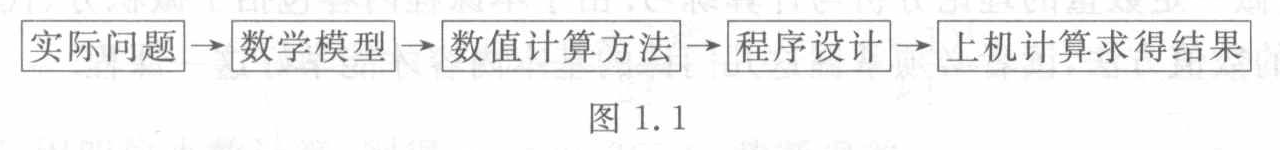
\includegraphics[width=0.85\linewidth,height=\textheight,keepaspectratio,alt={图1.1（原图裁切）}]{verified/assets/ch01/fig-1-1.png}

图1.1。图中各矩形框依次以向右箭头相连：实际问题 → 数学模型 → 数值计算方法 → 程序设计 → 上机计算求得结果。

由实际问题的提出到上机计算求得结果, 整个过程都可看作应用数学的研究对象. 如果细分的话, 针对实际问题应用有关科学知识和数学理论建立数学模型这一过程, 通常作为应用数学的研究对象, 而根据数学模型提出求解的数值计算方法直到编出程序上机算出结果这一过程, 则是计算数学的研究对象, 也是数值分析的研究对象. 因此, 数值分析就是研究用计算机解决数学问题的数值方法及其理论, 它的内容包括函数的数值逼近、数值微分与数值积分、非线性方程数值解、数值线性代数、微分方程数值解等, 它们都是以数学问题为研究对象的. 因此, 数值分析是数学的一个分支, 只是它不像纯数学那样只研究数学本身的理论, 而是把理论与计算紧密结合起来, 着重研究数学问题的数值方法及其理论.

数值分析也称为计算方法, 但不应片面地将它理解为各种数值方法的简单罗列和堆积. 同数学分析一样, 它内容丰富, 研究方法深刻, 有自身理论体系的课程, 既有纯数学的高度抽象性与严密科学性的特点, 又有应用的广泛性与实际试验的高度技术性的特点, 是一门与计算机应用密切结合的、实用性很强的数学课程. 它与纯数学课程不同, 例如, 在考虑线性方程组数值解时, ``线性代数''中只介绍解存在的唯一性及有关理论和精确解法, 运用这些理论和方法, 无法在计算机上求解上百个未知数的方程组, 更不用说求解十几万个未知数的方程组了. 求解这类问题还应根据方程特点, 研究适合计算机使用的、满足精度要求的、计算省时间的有效算法及其相关的理

\begin{quote}
校注（agent 补充）：本页末尾``理''字与下一页开头``论''字相接。
\end{quote}

\clearpage

原书 PDF 页 15；印刷页码 2。

\href{source-images/pdf-015.jpeg}{查看原页}

论;在实现这些算法时往往还要根据计算机容量、字长、速度等指标,研究具体求解步骤和程序设计技巧;有的方法在理论上虽不够严格,但通过实际计算、对比分析等手段,只要能证明它们是行之有效的方法,也应采用.这些就是数值分析具有的特点,概括起来有四点.

第一,面向计算机,要根据计算机特点提供实际可行的有效算法,即算法只能包括加、减、乘、除运算和逻辑运算,它们都是计算机能直接处理的.

第二,有可靠的理论分析,能任意逼近并达到精度要求,对近似算法要保证收敛性和数值稳定性,还要对误差进行分析.这些都要建立在相应数学理论的基础上.

第三,有好的计算复杂性.时间复杂性好是指节省时间,空间复杂性好是指节省存储量,这也是建立算法要研究的问题,它关系到算法能否在计算机上实现.

第四,有数值实验.任何一个算法,除了从理论上要满足上述三点外,还要通过数值实验证明它是行之有效的.

根据``数值分析''的特点,学习时首先要注意掌握方法的基本原理和思想,要注意方法处理的技巧及其与计算机的结合,要重视误差分析、收敛性及稳定性的基本理论;其次,要通过例子,学习使用各种数值方法解决实际计算问题;最后,为了掌握本课程的内容,还应做一定数量的理论分析与计算练习.由于本课程内容包括了微积分、代数、常微分方程的数值方法,读者必须掌握这几门课的基本内容才能学好这一课程.

\subsubsection{1.2 误差来源与误差分析的重要性}\label{ch01-ux8befux5deeux6765ux6e90ux4e0eux8befux5deeux5206ux6790ux7684ux91cdux8981ux6027}

用计算机解决科学计算问题首先要建立数学模型,它是对被描述的实际问题进行抽象、简化而得到的,因而是近似的.我们把数学模型与实际问题之间出现的这种误差称为模型误差.只有实际问题提法正确,建立数学模型时又抽象、简化得合理,才能得到好的结果.由于这种误差难以用数量表示,通常都假定数学模型是合理的,这种误差可忽略不计,在``数值分析''中不予讨论.在数学模型中往往还有一些根据观测得到的物理量,如温度、长度、电压等,这些参量显然也包含误差.这种由观测产生的误差称为观测误差,在``数值分析''中也不讨论这种误差.数值分析只研究用数值方法求解数学模型产生的误差.

当数学模型不能得到精确解时,通常要用数值方法求它的近似解,其近似解与精确解之间的误差称为截断误差或方法误差.例如,当函数 \(f(x)\) 用 Taylor多项式

\[
P_n(x)=f(0)+\frac{f'(0)}{1!}x+\frac{f''(0)}{2!}x^2+\cdots+\frac{f^{(n)}(0)}{n!}x^n
\]

近似代替时,数值方法的截断误差是

\[
R_n(x)=f(x)-P_n(x)=\frac{f^{(n+1)}(\xi)}{(n+1)!}x^{n+1},\qquad \xi\text{ 在 }x\text{ 与 }0\text{ 之间}.
\]

\clearpage

原书 PDF 页 16；印刷页码 3。

\href{source-images/pdf-016.jpeg}{查看原页}

有了求解数学问题的计算公式以后，用计算机进行数值计算时，由于计算机的字长有限，原始数据在计算机上表示会产生误差，计算过程又可能产生新的误差，这种误差称为舍入误差，例如，用3.14159近似代替\(\pi\)，产生的误差

\[
R = \pi - 3.14159 = 0.0000026\cdots
\]

就是舍入误差. 在``数值分析''中除了研究数学问题的算法外，还要研究计算结果的误差是否满足精度要求，这就是误差估计问题. 本书主要讨论算法的截断误差与舍入误差，对舍入误差通常只作一些定性分析. 下面举例说明误差分析的重要性.

\textbf{例1.1} 计算 \(I_n = \mathrm{e}^{-1} \int_{0}^{1} x^n \mathrm{e}^{x} \mathrm{d}x (n = 0,1,\cdots)\)，并估计误差.

\textbf{解} 由分部积分可得计算 \(I_n\) 的递推公式

\[
I_n = 1 - n I_{n-1} \quad (n = 1,2,\cdots), \tag{1.2.1}
\]

\[
I_0 = \mathrm{e}^{-1} \int_{0}^{1} \mathrm{e}^{x} \mathrm{d}x = 1 - \mathrm{e}^{-1}.
\]

若计算出 \(I_0\)，代入式(1.2.1)，可逐次求出 \(I_1, I_2, \cdots\) 的值. 要算出 \(I_0\) 就要先计算 \(\mathrm{e}^{-1}\)，若用 Taylor多项式展开部分和

\[
\mathrm{e}^{-1} \approx 1 + (-1) + \frac{(-1)^2}{2!} + \cdots + \frac{(-1)^k}{k!},
\]

并取 \(k=7\)，用四位小数计算，则得 \(\mathrm{e}^{-1} \approx 0.3679\)，截断误差

\[
R_7 = |\mathrm{e}^{-1} - 0.3679| \leqslant \frac{1}{8!} < \frac{1}{4} \times 10^{-4}.
\]

计算过程中小数点后第五位的数字按四舍五入原则舍入，由此产生的舍入误差这里先不讨论. 当初值取为 \(I_0 \approx 0.6321 = \tilde{I}_0\) 时，用式(1.2.1)递推的计算公式为 方案(A)

\[
\begin{cases}
\tilde{I}_0 = 0.6321, \\
\tilde{I}_n = 1 - n \tilde{I}_{n-1} \quad (n = 1,2,\cdots).
\end{cases}
\]

计算结果如表1.1的 \(\tilde{I}_n\) 列所示. 用 \(\tilde{I}_0\) 近似 \(I_0\) 产生的误差 \(E_0 = I_0 - \tilde{I}_0\) 就是初值误差，它对后面计算结果是有影响的.

表1.1

{\def\LTcaptype{none} % do not increment counter
\begin{longtable}[]{@{}
  >{\raggedright\arraybackslash}p{(\linewidth - 10\tabcolsep) * \real{0.1667}}
  >{\raggedright\arraybackslash}p{(\linewidth - 10\tabcolsep) * \real{0.1667}}
  >{\raggedright\arraybackslash}p{(\linewidth - 10\tabcolsep) * \real{0.1667}}
  >{\raggedright\arraybackslash}p{(\linewidth - 10\tabcolsep) * \real{0.1667}}
  >{\raggedright\arraybackslash}p{(\linewidth - 10\tabcolsep) * \real{0.1667}}
  >{\raggedright\arraybackslash}p{(\linewidth - 10\tabcolsep) * \real{0.1667}}@{}}
\toprule\noalign{}
\begin{minipage}[b]{\linewidth}\raggedright
\(n\)
\end{minipage} & \begin{minipage}[b]{\linewidth}\raggedright
\(\tilde{I}_n\) (用方案(A)计算)
\end{minipage} & \begin{minipage}[b]{\linewidth}\raggedright
\(I_n^*\) (用方案(B)计算)
\end{minipage} & \begin{minipage}[b]{\linewidth}\raggedright
\(n\)
\end{minipage} & \begin{minipage}[b]{\linewidth}\raggedright
\(\tilde{I}_n\) (用方案(A)计算)
\end{minipage} & \begin{minipage}[b]{\linewidth}\raggedright
\(I_n^*\) (用方案(B)计算)
\end{minipage} \\
\midrule\noalign{}
\endhead
\bottomrule\noalign{}
\endlastfoot
0 & 0.6321 & 0.6321 & 5 & 0.1480 & 0.1455 \\
1 & 0.3679 & 0.3679 & 6 & 0.1120 & 0.1268 \\
2 & 0.2642 & 0.2643 & 7 & 0.2160 & 0.1121 \\
3 & 0.2074 & 0.2073 & 8 & -0.728 & 0.1035 \\
4 & 0.1704 & 0.1708 & 9 & 7.552 & 0.0684 \\
\end{longtable}
}

\clearpage

原书 PDF 页 17；印刷页码 4。

\href{source-images/pdf-017.jpeg}{查看原页}

从表1.1可以看到，\(\tilde{I}_8\) 出现负值，这与一切 \(I_n > 0\) 相矛盾. 实际上，由积分估值得

\[
\frac{e^{-1}}{n+1} = e^{-1}\left(\min_{0 \leqslant x \leqslant 1} e^x\right)\int_0^1 x^n \mathrm{d}x < I_n < e^{-1}\left(\max_{0 \leqslant x \leqslant 1} e^x\right)\int_0^1 x^n \mathrm{d}x = \frac{1}{n+1}. \tag{1.2.2}
\]

因此，当 \(n\) 较大时，用 \(\tilde{I}_n\) 近似 \(I_n\) 显然是不正确的. 这里，计算公式与每步计算都是正确的，那么，是什么原因使计算结果错误呢？主要就是初值 \(\tilde{I}_0\) 有误差 \(E_0 = I_0 - \tilde{I}_0\)， 由此引起以后各步计算的误差 \(E_n = I_n - \tilde{I}_n\) 满足关系 \(E_n = -nE_{n-1}(n=1,2,\cdots)\). 容易推得

\[
E_n = (-1)^n n! E_0,
\]

这说明 \(\tilde{I}_0\) 有误差 \(E_0\)，则 \(\tilde{I}_n\) 就是 \(E_0\) 的 \(n!\) 倍误差. 例如，\(n=8\)，若 \(|E_0| = \frac{1}{2} \times 10^{-4}\)，则 \(|E_8| = 8! \times |E_0| > 2\). 这就说明 \(\tilde{I}_8\) 完全不能近似 \(I_8\) 了. 我们现在换一种计算方案. 由式(1.2.2)取 \(n=9\)，得

\[
\frac{e^{-1}}{10} < I_9 < \frac{1}{10},
\]

粗略取 \(I_9 \approx \frac{1}{2}\left(\frac{1}{10} + \frac{e^{-1}}{10}\right) = 0.0684 = I_9^*\)， 然后将式(1.2.1)倒过来算，即由 \(I_9^*\) 算出 \(I_8^*, I_7^*, \cdots, I_1^*\)，公式为 方案(B)

\[
\begin{cases} I_9^* = 0.0684, \\ I_{n-1}^* = \frac{1}{n}(1 - I_n^*) \quad (n = 9, 8, \cdots, 1). \end{cases}
\]

计算结果如表1.1中的 \(I_n^*\) 列所示. 可以发现，\(I_0^*\) 与 \(I_0\) 的误差不超过 \(10^{-4}\). 由于 \(|E_0^*| = \frac{1}{n!}|E_n^*|, E_0^*\) 比 \(E_n^*\) 缩小了 \(n!\) 倍，因此，尽管 \(E_9^*\) 较大，但由于误差逐步缩小，故可用 \(I_n^*\) 近似 \(I_n\). 反之，当用方案(A)计算时，尽管初值 \(\tilde{I}_0\) 相当准确，但由于误差传播是逐步扩大的，因而计算结果不可靠. 此例说明，在数值计算中如不注意误差分析，用了类似于方案(A)的计算公式，就会出现``差之毫厘，失之千里''的错误结果. 尽管数值计算中估计误差比较困难，但仍应重视计算过程中的误差分析.

\subsubsection{1.3 误差的基本概念}\label{ch01-ux8befux5deeux7684ux57faux672cux6982ux5ff5}

\paragraph{1.3.1 误差与误差限}\label{ch01-ux8befux5deeux4e0eux8befux5deeux9650}

\textbf{定义1.1} 设 \(x\) 为准确值，\(x^*\) 为 \(x\) 的一个近似值，称 \(e^* = x^* - x\) 为近似值的绝

\begin{quote}
校注（agent 补充）：本页定义1.1末尾``绝''字与下一页``对误差''相接。
\end{quote}

\begin{quote}
校注（agent 补充，CH01-E001）：原书写``则 \(\tilde{I}_n\) 就是 \(E_0\) 的 \(n!\) 倍误差''，此处照录。由上式 \(E_n=(-1)^n n!E_0\) 可知，应理解为近似值 \(\tilde{I}_n\) 的误差绝对值为初值误差绝对值的 \(n!\) 倍；疑为原书表述不严谨，不是 OCR 错误。
\end{quote}

\clearpage

原书 PDF 页 18；印刷页码 5。

\href{source-images/pdf-018.jpeg}{查看原页}

对误差, 简称误差.

注意, 这样定义的误差 \(e^*\) 可正可负, 当绝对误差为正时近似值偏大, 叫做强近似值; 当绝对误差为负时近似值偏小, 叫做弱近似值.

通常, 我们不能算出准确值 \(x\), 也不能算出误差 \(e^*\) 的准确值, 只能根据测量工具或计算情况估计出误差的绝对值不超过某正数 \(\varepsilon^*\), 也就是误差绝对值的一个上界. \(\varepsilon^*\) 叫做近似值的误差限, 它总是正数. 例如, 用毫米刻度的米尺测量一长度 \(x\) (单位: mm, 下同), 读出和该长度接近的刻度 \(x^*\), \(x^*\) 是 \(x\) 的近似值, 它的误差限是 0.5, 于是 \(|x^* - x| \leqslant 0.5\); 如读出的长度为 765, 则有 \(|765 - x| \leqslant 0.5\). 从该不等式仍不知道准确的 \(x\) 是多少, 但知道 \(764.5 \leqslant x \leqslant 765.5\), 说明 \(x\) 在区间 \([764.5, 765.5]\) 上.

对于一般情形, \(|x^* - x| \leqslant \varepsilon^*\), 即 \(x^* - \varepsilon^* \leqslant x \leqslant x^* + \varepsilon^*\), 这个不等式有时也表示为

\[
x = x^* \pm \varepsilon^*.
\]

\paragraph{1.3.2 相对误差与相对误差限}\label{ch01-ux76f8ux5bf9ux8befux5deeux4e0eux76f8ux5bf9ux8befux5deeux9650}

误差限的大小还不能完全表示近似值的好坏. 例如, 有两个量 \(x = 10 \pm 1, y = 1000 \pm 5\), 则

\[
x^* = 10, \varepsilon_x^* = 1, y^* = 1000, \varepsilon_y^* = 5.
\]

虽然 \(\varepsilon_y^*\) 比 \(\varepsilon_x^*\) 大 4 倍, 但 \(\frac{\varepsilon_y^*}{y^*} = \frac{5}{1000} = 0.5\%\) 比 \(\frac{\varepsilon_x^*}{x^*} = \frac{1}{10} = 10\%\) 要小得多, 这说明 \(y^*\) 近似 \(y\) 的程度比 \(x^*\) 近似 \(x\) 的程度要好得多. 所以, 除考虑误差的大小外, 还应考虑准确值 \(x\) 本身的大小. 近似值的误差 \(e^*\) 与准确值 \(x\) 的比值

\[
\frac{e^*}{x} = \frac{x^* - x}{x}
\]

称为近似值 \(x^*\) 的相对误差, 记作 \(e_r^*\).

在实际计算中, 由于真值 \(x\) 总是不知道的, 通常取

\[
e_r^* = \frac{e^*}{x^*} = \frac{x^* - x}{x^*}
\]

作为 \(x^*\) 的相对误差, 条件是 \(e_r^* = \frac{e^*}{x^*}\) 较小, 此时

\[
\frac{e^*}{x} - \frac{e^*}{x^*} = \frac{e^* (x^* - x)}{x^* x} = \frac{(e^*)^2}{x^* (x^* - e^*)} = \frac{(e^* / x^*)^2}{1 - (e^* / x^*)}
\]

是 \(e_r^*\) 的二次方项级, 故可忽略不计.

相对误差也可正可负, 它的绝对值上界叫做相对误差限, 记作 \(\varepsilon_r^*, \varepsilon_r^* = \frac{\varepsilon^*}{|x^*|}\).

根据定义, \(\frac{\varepsilon_x^*}{|x^*|} = 10\%\) 与 \(\frac{\varepsilon_y^*}{|y^*|} = 0.5\%\) 分别为 \(x\) 与 \(y\) 的相对误差限, 可见 \(y^*\) 近似 \(y\) 的程度比 \(x^*\) 近似 \(x\) 的程度好.

\clearpage

原书 PDF 页 19；印刷页码 6。

\href{source-images/pdf-019.jpeg}{查看原页}

\paragraph{1.3.3 有效数字}\label{ch01-ux6709ux6548ux6570ux5b57}

当准确值 \(x\) 有多位数时，常常按四舍五入的原则得到 \(x\) 的前几位近似值 \(x^*\). 例如

\[
x = \pi = 3.14159265\cdots,
\]

取前三位，\(x_3^* = 3.14, \varepsilon_3^* \leqslant 0.002\)；取前五位，\(x_5^* = 3.1416, \varepsilon_5^* \leqslant 0.000008\)：它们的误差都不超过末位数字的半个单位，即

\[
|\pi - 3.14| \leqslant \frac{1}{2} \times 10^{-2}, \quad |\pi - 3.1416| \leqslant \frac{1}{2} \times 10^{-4}.
\]

若近似值 \(x^*\) 的误差限是某一位的半个单位，该位到 \(x^*\) 的第一位非零数字共有 \(n\) 位，就说 \(x^*\) 有 \(n\) 位有效数字. 如取 \(x^* = 3.14\) 作 \(\pi\) 的近似值，\(x^*\) 就有三位有效数字；取 \(x^* = 3.1416\) 作 \(\pi\) 的近似值，\(x^*\) 就有五位有效数字. \(x^*\) 有 \(n\) 位有效数字可写成标准形式

\[
x^* = \pm 10^m \times (a_1 + a_2 \times 10^{-1} + \cdots + a_n \times 10^{-(n-1)}), \tag{1.3.1}
\]

其中，\(a_1\) 是 1 到 9 中的一个数字；\(a_2, \cdots, a_n\) 是 0 到 9 中的一个数字；\(m\) 为整数，且

\[
|x - x^*| \leqslant \frac{1}{2} \times 10^{m-n+1}. \tag{1.3.2}
\]

\textbf{例1.2} 按四舍五入原则写出下列各数具有五位有效数字的近似数： 187.932 5，0.037 855 51，8.000 033，2.718 281 8.

\textbf{解} 按定义，上述各数具有五位有效数字的近似数分别是 187.93，0.037 856，8.000 0，2.718 3.

注意 \(x = 8.000033\) 的五位有效数字近似数是 8.0000 而不是 8，因为 8 只有一位有效数字.

\textbf{例1.3} 重力常数 \(g\)，如果以 \(\mathrm{m/s^2}\) 为单位，\(g \approx 9.80 \text{ m/s}^2\)；若以 \(\mathrm{km/s^2}\) 为单位，\(g \approx 0.00980 \text{ km/s}^2\)，它们都具有三位有效数字. 按第一种写法，有

\[
|g - 9.80| \leqslant \frac{1}{2} \times 10^{-2},
\]

据式(1.3.1)，这里 \(m=0, n=3\)；按第二种写法，有

\[
|g - 0.00980| \leqslant \frac{1}{2} \times 10^{-5},
\]

这里 \(m=-3, n=3\). 它们虽然写法不同，但都具有三位有效数字. 至于绝对误差限，由于单位不同，结果也不同，\(\varepsilon_1^* = \frac{1}{2} \times 10^{-2} \text{ m/s}^2, \varepsilon_2^* = \frac{1}{2} \times 10^{-5} \text{ km/s}^2\)，而相对误差都是

\[
\varepsilon_r^* = 0.005/9.80 = 0.000005/0.00980.
\]

注意 相对误差与相对误差限是无量纲的，而绝对误差与误差限是有量纲的. 例 1.3 说明有效位数与小数点后有多少位数无关. 然而，从式(1.3.2)可得到具

\begin{quote}
校注（agent 补充）：本页末尾``具''字与下一页``有 \(n\) 位有效数字''相接。
\end{quote}

\clearpage

原书 PDF 页 20；印刷页码 7。

\href{source-images/pdf-020.jpeg}{查看原页}

有 \(n\) 位有效数字的近似数 \(x^*\), 其绝对误差限为

\[
\varepsilon^* = \frac{1}{2} \times 10^{m-n+1},
\]

在 \(m\) 相同的情况下, \(n\) 越大, \(10^{m-n+1}\) 越小, 故有效位数越多, 绝对误差限越小. 关于有效数字与相对误差限的关系, 有如下定理.

\textbf{定理1.1} 对于用式(1.3.1)表示的近似数 \(x^*\), 若 \(x^*\) 具有 \(n\) 位有效数字, 则其相对误差限为

\[
\varepsilon_r^* \leqslant \frac{1}{2a_1} \times 10^{-(n-1)};
\]

反之, 若 \(x^*\) 的相对误差限 \(\varepsilon_r^* \leqslant \frac{1}{2(a_1+1)} \times 10^{-(n-1)}\), 则 \(x^*\) 至少具有 \(n\) 位有效数字.

\textbf{证明} 由式(1.3.1)可得 \(a_1 \times 10^m \leqslant |x^*| \leqslant (a_1+1) \times 10^m\), 当 \(x^*\) 有 \(n\) 位有效数字时, 有

\[
\varepsilon_r^* = \frac{|x-x^*|}{|x^*|} \leqslant \frac{0.5 \times 10^{m-n+1}}{a_1 \times 10^m} = \frac{1}{2a_1} \times 10^{-n+1};
\]

反之, 有

\[
|x-x^*| = |x^*| \varepsilon_r^* \leqslant (a_1+1) \times 10^m \times \frac{1}{2(a_1+1)} \times 10^{-n+1} = 0.5 \times 10^{m-n+1},
\]

故 \(x^*\) 有 \(n\) 位有效数字. 证毕.

定理 1.1 说明, 有效位数越多, 相对误差限越小.

\textbf{例1.4} 要使 \(\sqrt{20}\) 的近似值的相对误差限小于 \(0.1\%\), 要取几位有效数字?

\textbf{解} 由定理 1.1 知

\[
\varepsilon_r^* \leqslant \frac{1}{2a_1} \times 10^{-n+1}.
\]

由 \(\sqrt{20} = 4.4 \dots\) 知, \(a_1 = 4\), 故只要取 \(n=4\), 就有

\[
\varepsilon_r^* \leqslant 0.125 \times 10^{-3} < 10^{-3} = 0.1\%,
\]

即只要对 \(\sqrt{20}\) 的近似值取四位有效数字, 其相对误差限就小于 \(0.1\%\), 此时

\[
\sqrt{20} \approx 4.472.
\]

\paragraph{1.3.4 数值运算的误差估计}\label{ch01-ux6570ux503cux8fd0ux7b97ux7684ux8befux5deeux4f30ux8ba1}

两个近似数 \(x_1^*\) 与 \(x_2^*\), 其误差限分别为 \(\varepsilon(x_1^*)\) 及 \(\varepsilon(x_2^*)\), 它们进行加、减、乘、除运算得到的误差限分别为

\[
\varepsilon(x_1^* \pm x_2^*) = \varepsilon(x_1^*) + \varepsilon(x_2^*),
\]

\[
\varepsilon(x_1^* x_2^*) \approx |x_1^*| \varepsilon(x_2^*) + |x_2^*| \varepsilon(x_1^*),
\]

\[
\varepsilon\left(\frac{x_1^*}{x_2^*}\right) \approx \frac{|x_1^*| \varepsilon(x_2^*) + |x_2^*| \varepsilon(x_1^*)}{|x_2^*|^2} \quad (x_2^* \neq 0).
\]

更一般的情况是, 当自变量有误差时, 计算函数值也会产生误差, 其误差限可利

\begin{quote}
校注（agent 补充）：本页末尾``可利''与下一页``用函数的 Taylor 展开式进行估计''相接。
\end{quote}

\clearpage

原书 PDF 页 21；印刷页码 8。

\href{source-images/pdf-021.jpeg}{查看原页}

用函数的 Taylor 展开式进行估计。设 \(f(x)\) 是一元函数，\(x\) 的近似值为 \(x^*\)，以 \(f(x^*)\) 近似 \(f(x)\)，其误差限记作 \(\varepsilon(f(x^*))\)，可用 Taylor 展开

\[
f(x)-f(x^*)=f'(x^*)(x-x^*)+\frac{f''(\xi)}{2}(x-x^*)^2,
\]

\(\xi\) 介于 \(x,x^*\) 之间。取绝对值得

\[
|f(x)-f(x^*)|\leqslant |f'(x^*)|\varepsilon(x^*)+\frac{|f''(\xi)|}{2}\varepsilon^2(x^*).
\]

假定 \(f'(x^*)\) 与 \(f''(x^*)\) 的比值不太大，可忽略 \(\varepsilon(x^*)\) 的高阶项，于是可得计算函数的误差限为

\[
\varepsilon(f(x^*))\approx |f'(x^*)|\varepsilon(x^*).
\]

当 \(f\) 为多元函数时计算 \(A=f(x_1,x_2,\cdots,x_n)\)，如果 \(x_1,x_2,\cdots,x_n\) 的近似值为 \(x_1^*,x_2^*,\cdots,x_n^*\)，则 \(A\) 的近似值为 \(A^*=f(x_1^*,x_2^*,\cdots,x_n^*)\)，于是函数值 \(A^*\) 的误差 \(e(A^*)\) 由 Taylor 展开，得

\[
\begin{aligned}
e(A^*)&=A^*-A=f(x_1^*,x_2^*,\cdots,x_n^*)-f(x_1,x_2,\cdots,x_n)\\
&\approx\sum_{k=1}^{n}\left(\frac{\partial f(x_1^*,x_2^*,\cdots,x_n^*)}{\partial x_k}\right)(x_k^*-x_k)
=\sum_{k=1}^{n}\left(\frac{\partial f}{\partial x_k}\right)^*e_k^*,
\end{aligned}
\]

于是误差限为

\[
\varepsilon(A^*)\approx\sum_{k=1}^{n}\left|\left(\frac{\partial f}{\partial x_k}\right)^*\right|\varepsilon(x_k^*);
\tag{1.3.3}
\]

而 \(A^*\) 的相对误差限为

\[
\varepsilon_r^*=\varepsilon_r(A^*)=\frac{\varepsilon(A^*)}{|A^*|}\approx\sum_{k=1}^{k}\left|\left(\frac{\partial f}{\partial x_k}\right)^*\right|\frac{\varepsilon(x_k^*)}{|A^*|}.
\tag{1.3.4}
\]

\textbf{例1.5} 已测得某场地长 \(l\) 的值为 \(l^*=110\ \mathrm{m}\)，宽 \(d\) 的值为 \(d^*=80\ \mathrm{m}\)，已知 \(|l-l^*|\leqslant 0.2\ \mathrm{m}\)，\(|d-d^*|\leqslant 0.1\ \mathrm{m}\)，试求面积 \(S=ld\) 的绝对误差限与相对误差限。

\textbf{解} 因 \(S=ld,\dfrac{\partial S}{\partial l}=d,\dfrac{\partial S}{\partial d}=l\)，由式(1.3.3)知

\[
\varepsilon(S^*)\approx\left|\left(\frac{\partial S}{\partial l}\right)^*\right|\varepsilon(l^*)+\left|\left(\frac{\partial S}{\partial d}\right)^*\right|\varepsilon(d^*),
\]

其中

\[
\left(\frac{\partial S}{\partial l}\right)^*=d^*=80\ \mathrm{m},\quad
\left(\frac{\partial S}{\partial d}\right)^*=l^*=110\ \mathrm{m},
\]

而

\[
\varepsilon(l^*)=0.2\ \mathrm{m},\quad\varepsilon(d^*)=0.1\ \mathrm{m},
\]

于是绝对误差限为

\[
\varepsilon(S^*)\approx(80\times0.2+110\times0.1)\ \mathrm{m}^2=27\ \mathrm{m}^2;
\]

相对误差限为

\[
\varepsilon_r(S^*)=\frac{\varepsilon(S^*)}{|S^*|}=\frac{\varepsilon(S^*)}{l^*d^*}\approx\frac{27}{8800}=0.31\%.
\]

\begin{quote}
校注（agent 补充，CH01-E002）：式(1.3.4)原图的求和上限清楚印为 \(k\)，本页保留 \(\sum_{k=1}^{k}\)。由函数有 \(n\) 个变量以及紧前式(1.3.3)的上限 \(n\) 判断，疑为原书将 \(n\) 误排为 \(k\)。OCR 候选写成 \(n\)，不能据此静默改原书。
\end{quote}

\begin{quote}
校注（agent 补充，CH01-E003）：原书关于可忽略高阶项的条件写为``\(f'(x^*)\) 与 \(f''(x^*)\) 的比值不太大''，此处照录。若意在使二阶项相对一阶项较小，应控制 \(|f''(\xi)|\varepsilon(x^*)/(2|f'(x^*)|)\)（在分母非零时）；原句疑有比值顺序或条件表述问题，不是 OCR 错误。
\end{quote}

\clearpage

原书 PDF 页 22；印刷页码 9。

\href{source-images/pdf-022.jpeg}{查看原页}

\subsubsection{1.4 数值运算中误差分析的方法与原则}\label{ch01-ux6570ux503cux8fd0ux7b97ux4e2dux8befux5deeux5206ux6790ux7684ux65b9ux6cd5ux4e0eux539fux5219}

数值运算中的误差分析是个很重要而复杂的问题，上节讨论了不精确数据运算结果的误差限，它只适用于简单情形。然而实际工程或科学计算问题往往要运算千万次，而且每步运算都有误差，但是每步都作误差分析是不可能的，也是不科学的。这是因为，误差积累有正有负，绝对值有大有小，都按最坏情况估计误差限得到的结果比实际误差大得多，这种保守的误差估计不反映实际误差积累。考虑到误差分布的随机性，有人用概率统计方法，将数据和运算中的舍入误差视为适合某种分布的随机变量，然后确定计算结果的误差分布，这样得到的误差估计更接近实际，这种方法称为概率分析法。

20世纪60年代以后，有人对舍入误差分析提出了一些新方法，但都不是十分有效。目前解决这一问题的办法，常常是针对不同类型问题逐个进行分析。由于定量分析常常是很困难的，因此对误差积累问题进行定性分析就有重要意义，这就要引入数值稳定性概念。运算过程舍入误差不增长的计算公式是数值稳定的，否则是不稳定的。如在例1.1给出的两种计算方案中，方案(A)由于初值有误差，在计算过程中这一误差逐渐增大，故是数值不稳定的；而方案(B)虽然初值也有误差，但计算过程误差不增长，故是数值稳定的。研究一个计算公式是否稳定，只要假定初始值有误差 \(\varepsilon_0\)，中间不再产生新误差，考察由 \(\varepsilon_0\) 引起的误差积累是否增长，如不增长就认为是稳定的，否则是不稳定的。对于稳定的计算公式，不具体估计舍入误差积累也可相信它是可用的，误差限不会太大；而不稳定的公式通常就不能使用，如要使用，其计算步数也只能很少，并且注意对误差积累进行控制。在本课程中，对各种计算过程都只研究它的稳定性，而不具体估计舍入误差。这里只提出数值运算中应注意的若干原则，它有助于鉴别计算结果的可靠性并防止误差危害现象的产生。

\paragraph{1.4.1 要避免除数绝对值远远小于被除数绝对值的除法}\label{ch01-ux8981ux907fux514dux9664ux6570ux7eddux5bf9ux503cux8fdcux8fdcux5c0fux4e8eux88abux9664ux6570ux7eddux5bf9ux503cux7684ux9664ux6cd5}

用绝对值小的数作除数，舍入误差会增大，如计算 \(\frac{x}{y}\)，若 \(0 < |y| \ll |x|\)，则可能对计算结果带来严重影响，应尽量避免。

\textbf{例1.6} 线性方程组 \(\begin{cases} 0.00001x_1 + x_2 = 1 \\ 2x_1 + x_2 = 2 \end{cases}\) 的准确解为 \[
x_1 = \frac{200000}{399999} = 0.50000125,
\] \[
x_2 = \frac{199998}{199999} = 0.999995.
\]

\begin{quote}
校注（agent 补充，CH01-E004）：原书把例1.6的 \(x_1\) 写成 \(200000/399999=0.50000125\)，此处照录。由原方程两式相减，\((2-0.00001)x_1=1\)，所以 \(x_1=100000/199999\approx0.5000025000125\)；原书所列 \(x_2=199998/199999\) 与后一结果一致。疑为原书 \(x_1\) 分式及小数有误，不是 OCR 错误。
\end{quote}

\clearpage

原书 PDF 页 23；印刷页码 10。

\href{source-images/pdf-023.jpeg}{查看原页}

现在四位浮点十进制数（仿机器实际计算）下用消去法求解，上述方程组写成

\[
\begin{cases} 10^{-4} \times 0.1000x_1 + 10^1 \times 0.1000x_2 = 10^1 \times 0.1000, \\ 10^1 \times 0.2000x_1 + 10^1 \times 0.1000x_2 = 10^1 \times 0.2000. \end{cases}
\]

若用 \((10^{-4} \times 0.1000)/2\) 除以第一个方程然后减去第二个方程，则出现了用小数除以大数的现象，得

\[
\begin{cases} 10^{-4} \times 0.1000x_1 + 10^1 \times 0.1000x_2 = 10^1 \times 0.1000, \\ 10^6 \times 0.2000x_2 = 10^6 \times 0.2000, \end{cases}
\]

由此解出 \(x_1=0, x_2=10^1 \times 0.1000=1\)，显然严重失真. 若反过来用第二个方程消去第一个方程中含 \(x_1\) 的项，则避免了大数被小数除的现象，得

\[
\begin{cases} 10^6 \times 0.1000x_2 = 10^6 \times 0.1000, \\ 10^1 \times 0.2000x_1 + 10^1 \times 0.1000x_2 = 10^1 \times 0.2000, \end{cases}
\]

由此求得相当好的近似解 \(x_1=0.5000, x_2=10^1 \times 0.1000\).

\paragraph{1.4.2 要避免两相近数相减}\label{ch01-ux8981ux907fux514dux4e24ux76f8ux8fd1ux6570ux76f8ux51cf}

在数值计算中，两相近数相减会导致有效数字严重损失.例如，\(x=532.65, y=532.52\)都有五位有效数字，但 \(x-y=0.13\)只有两位有效数字.必须尽量避免出现这类运算，最好是改变计算方法，防止这种现象产生.现举例说明.

\textbf{例1.7} 计算 \(A=10^7(1-\cos 2^\circ)\).

\textbf{解} 由于 \(\cos 2^\circ=0.9994\)，直接计算，得

\[
A=10^7(1-\cos 2^\circ)=10^7(1-0.9994)=6 \times 10^3,
\]

只有一位有效数字；若利用 \(1-\cos x=2\sin^2\frac{x}{2}\) 计算，则有

\[
A=10^7(1-\cos 2^\circ)=2 \times (\sin 1^\circ)^2 \times 10^7=6.13 \times 10^3,
\]

具有三位有效数字（这里 \(\sin 1^\circ=0.0175\)）.

例1.7 说明，可通过改变计算公式避免或减少有效数字的损失.类似地，如果 \(x_1\) 和 \(x_2\) 很接近，则

\[
\lg x_1-\lg x_2=\lg \frac{x_1}{x_2}.
\]

用右端算式，有效数字就不会损失.当 \(x\) 很大时，有

\[
\sqrt{x+1}-\sqrt{x}=\frac{1}{\sqrt{x+1}+\sqrt{x}},
\]

都用右端算式代替左端.一般情况下，当 \(f(x)\approx f(x^*)\) 时，可用 Taylor 展开

\[
f(x)-f(x^*)=f'(x^*) (x-x^*)+\frac{f''(x^*)}{2} (x-x^*)^2+\cdots,
\]

\begin{quote}
校注（agent 补充）：本页末尾 Taylor 展开后的讨论续下页。
\end{quote}

\begin{quote}
校注（agent 补充，CH01-E005）：例1.6续文原书写``用小数除以大数''，并在第二种消去结果的首行两侧印 \(10^6\)，此处均照录。按上下文，第一种操作是将第一方程除以小量 \((10^{-4}\times0.1000)/2\)；第二种操作直接以 \(R_1-0.000005R_2\) 消去，四位浮点结果应得到 \(10^1\times0.1000x_2=10^1\times0.1000\)。原印 \(10^6\) 的等式虽可通过两侧再同乘 \(10^5\) 得到，但原文没有该缩放步骤；上述措辞和指数均列为疑误，未静默修改。
\end{quote}

\begin{quote}
校注（agent 补充，CH01-E006）：例1.7原文``\(6.13\times10^3\)，具有三位有效数字''照录。独立数值复算 \(10^7(1-\cos2^\circ)\approx6091.729809\)，原列 \(6130\) 的误差约 \(38.270191\)，超过三位有效数字所对应的 \(5\)。以本章有效数字定义衡量，该``三位''判断存在问题；这不影响使用半角公式减轻相消的思路。
\end{quote}

\clearpage

原书 PDF 页 24；印刷页码 11。

\href{source-images/pdf-024.jpeg}{查看原页}

取右端的有限项近似左端. 如果无法改变算式, 则采用增加有效位数进行运算; 在计算机上则采用双倍字长运算, 但这要增加机器计算时间和多占内存单元.

\paragraph{1.4.3 要防止大数``吃掉''小数}\label{ch01-ux8981ux9632ux6b62ux5927ux6570ux5403ux6389ux5c0fux6570}

在数值运算中, 参加运算的数有时数量级相差很大, 而计算机位数有限, 如不注意运算次序就可能出现大数``吃掉''小数的现象, 影响计算结果的可靠性.

\textbf{例1.8} 在五位十进制计算机上, 计算

\[
A = 52\ 492 + \sum_{i=1}^{1000} \delta_i,
\]

其中 \(0.1 \leqslant \delta_i \leqslant 0.9\).

\textbf{解} 把运算的数写成规格化形式, 有

\[
A = 0.524\ 92 \times 10^5 + \sum_{i=1}^{1000} \delta_i.
\]

由于在计算机上计算时要对阶, 若取 \(\delta_i = 0.9\), 对阶时 \(\delta_i = 0.000\ 009 \times 10^5\), 在五位的计算机中表示为机器数 0, 因此

\[
A = 0.524\ 92 \times 10^5 + 0.000\ 009 \times 10^5 + \cdots + 0.000\ 009 \times 10^5
\]

\[
\triangleq 0.524\ 92 \times 10^5
\] （符号 \(\triangleq\) 表示机器中相等），

结果显然不可靠, 这是由运算中出现了大数 52 492``吃掉''小数 \(\delta_i\) 所造成的. 如果计算时先把数量级相同的 1 000 个 \(\delta_i\) 相加, 最后再加 52 492, 就不会出现大数``吃''小数的现象, 这时有

\[
0.1 \times 10^3 \leqslant \sum_{i=1}^{1000} \delta_i \leqslant 0.9 \times 10^3,
\]

\[
0.001 \times 10^5 + 0.524\ 92 \times 10^5 \leqslant A \leqslant 0.009 \times 10^5 + 0.524\ 92 \times 10^5,
\]

\[
52\ 592 \leqslant A \leqslant 53\ 392.
\]

\paragraph{1.4.4 注意简化计算步骤，减少运算次数}\label{ch01-ux6ce8ux610fux7b80ux5316ux8ba1ux7b97ux6b65ux9aa4ux51cfux5c11ux8fd0ux7b97ux6b21ux6570}

同样一个计算问题, 若能减少运算次数, 不但可节省计算机的计算时间, 还能减小舍入误差. 这是数值计算必须遵从的原则, 也是``数值分析''要研究的重要内容.

\textbf{例1.9} 计算 \(x^{255}\) 的值.

\textbf{解} 如果逐个相乘要用 254 次乘法, 但若写成

\[
x^{255} = x \cdot x^2 \cdot x^4 \cdot x^8 \cdot x^{16} \cdot x^{32} \cdot x^{64} \cdot x^{128},
\]

只要做 14 次乘法运算即可. 又如计算多项式

\[
P_n(x) = a_n x^n + a_{n-1} x^{n-1} + \cdots + a_1 x + a_0
\]

的值时, 若直接计算 \(a_k x^k\) 再逐项相加, 一共需做

\[
n + (n-1) + \cdots + 2 + 1 = \frac{n(n+1)}{2}
\]

\begin{quote}
校注（agent 补充）：本页末尾乘法次数公式的说明续下页``次乘法和 \(n\) 次加法''。
\end{quote}

\clearpage

原书 PDF 页 25；印刷页码 12。

\href{source-images/pdf-025.jpeg}{查看原页}

次乘法和 \(n\) 次加法. 若采用秦九韶算法

\[
\begin{cases} S_n = a_n, \\ S_k = xS_{k+1} + a_k & (k=n-1,n-2,\cdots,0), \\ P_n(x) = S_0, \end{cases} \tag{1.4.1}
\]

只要做 \(n\) 次乘法和 \(n\) 次加法就可算出 \(P_n(x)\) 的值.

在``数值分析''中, 这种节省计算次数的算法还有不少. 本书第 3 章介绍的 FFT 算法, 就是一个最成功的范例.

\subsubsection{小结}\label{ch01-ux5c0fux7ed3}

误差问题是``数值分析''中重要而又困难的课题. 本章只介绍误差基本概念与分析误差的若干原则, 这对学习本课程是必需的. 但作为工程或科学计算的误差问题则要复杂得多, 人们往往根据不同问题分门别类进行研究. 这里不作详细介绍, 有兴趣的读者请参看有关文献, 例如文献{[}1{]}、{[}2{]}等.

\subsubsection{习题}\label{ch01-ux4e60ux9898}

\begin{enumerate}
\def\labelenumi{\arabic{enumi}.}
\item
  设 \(x>0, x\) 的相对误差为 \(\delta\), 求 \(\ln x\) 的误差.
\item
  设 \(x\) 的相对误差为 \(2\%\), 求 \(x^n\) 的相对误差.
\item
  下列各数都是经过四舍五入得到的近似数, 即误差限不超过最后一位的半个单位, 试指出它们是几位有效数字:
\end{enumerate}

\[
x_1^* = 1.1021, x_2^* = 0.031, x_3^* = 385.6, x_4^* = 56.430, x_5^* = 7 \times 1.0.
\]

\begin{enumerate}
\def\labelenumi{\arabic{enumi}.}
\setcounter{enumi}{3}
\tightlist
\item
  利用式(1.3.3)求下列近似值的误差限:
\end{enumerate}

\begin{enumerate}
\def\labelenumi{(\arabic{enumi})}
\tightlist
\item
  \(x_1^* + x_2^* + x_4^*\), (2) \(x_1^* x_2^* x_3^*\), (3) \(x_2^* / x_4^*\), 其中 \(x_1^*, x_2^*, x_3^*, x_4^*\) 均为习题 3 所给的数.
\end{enumerate}

\begin{enumerate}
\def\labelenumi{\arabic{enumi}.}
\setcounter{enumi}{4}
\item
  计算球体积要使相对误差限为 \(1\%\), 问度量半径为 \(R\) 时允许的相对误差限是多少.
\item
  设 \(Y_0=28\), 按递推公式
\end{enumerate}

\[
Y_n = Y_{n-1} - \frac{1}{100} \sqrt{783} \quad (n=1,2,\cdots)
\]

计算到 \(Y_{100}\). 若取 \(\sqrt{783} \approx 27.982\) (五位有效数字), 试问计算 \(Y_{100}\) 将有多大误差.

\begin{enumerate}
\def\labelenumi{\arabic{enumi}.}
\setcounter{enumi}{6}
\item
  求方程 \(x^2-56x+1=0\) 的两个根, 使它至少具有四位有效数字 (\(\sqrt{783} \approx 27.982\)).
\item
  当 \(N\) 充分大时, 怎样求 \(\int_N^{N+1} \frac{1}{1+x^2} \mathrm{d}x\)?
\item
  正方形的边长大约为 \(100 \mathrm{~cm}\), 应怎样测量才能使其面积误差不超过 \(1 \mathrm{~cm}^2\)?
\item
  设 \(s=\frac{1}{2} g t^2\), 假定 \(g\) 是准确的, 而对 \(t\) 的测量有 \(\pm 0.1 \mathrm{~s}\) 的误差, 证明: 当 \(t\) 增加时 \(s\) 的绝对误差增大, 而相对误差却减小.
\item
  序列 \(\{y_n\}\) 满足递推关系 \(y_n=10y_{n-1}-1 (n=1,2,\cdots)\), 若 \(y_0=\sqrt{2} \approx 1.41\) (三位有效数字),
\end{enumerate}

\begin{quote}
校注（agent 补充）：习题3第五个数的原图清楚写为 \(x_5^*=7\times1.0\)，未作简化或改写。习题11在本页仅给出条件，题目后半句续下页。
\end{quote}

\clearpage

原书 PDF 页 26；印刷页码 13。

\href{source-images/pdf-026.jpeg}{查看原页}

计算到 \(y_{10}\) 时误差有多大？这个计算过程稳定吗？

\begin{enumerate}
\def\labelenumi{\arabic{enumi}.}
\setcounter{enumi}{11}
\tightlist
\item
  计算 \((\sqrt{2}-1)^6\), 取 \(\sqrt{2} \approx 1.4\), 利用下式计算, 哪一个得到的结果最好?
\end{enumerate}

\[
\frac{1}{(\sqrt{2}+1)^6}, \quad (3-2\sqrt{2})^3, \quad \frac{1}{(3+2\sqrt{2})^3}, \quad 99-70\sqrt{2}.
\]

\begin{enumerate}
\def\labelenumi{\arabic{enumi}.}
\setcounter{enumi}{12}
\tightlist
\item
  \(f(x)=\ln(x-\sqrt{x^2-1})\), 求 \(f(30)\) 的值. 求对数时误差有多大? 若改用另一等价公式
\end{enumerate}

\[
\ln(x-\sqrt{x^2-1})=-\ln(x+\sqrt{x^2+1})
\]

计算, 求对数时误差有多大?

\begin{enumerate}
\def\labelenumi{\arabic{enumi}.}
\setcounter{enumi}{13}
\item
  试用消元法解方程组 \(\begin{cases} x_1+10^{10}x_2=10^{10}, \\ x_1+x_2=2, \end{cases}\) 假定只用三位数计算, 结果是否可靠?
\item
  已知三角形面积 \(S=\frac{1}{2}ab\sin c\), 其中 \(c\) 为弧度, \(0<c<\frac{\pi}{2}\), 且测量 \(a, b, c\) 的误差分别为 \(\Delta a\), \(\Delta b\), \(\Delta c\). 证明面积的误差 \(\Delta S\) 满足
\end{enumerate}

\[
\left|\frac{\Delta S}{S}\right| \leqslant \left|\frac{\Delta a}{a}\right| + \left|\frac{\Delta b}{b}\right| + \left|\frac{\Delta c}{c}\right|.
\]

\begin{quote}
校注（agent 补充，CH01-E007）：习题13所谓``等价公式''的右端，原图清楚印为 \(-\ln(x+\sqrt{x^2+1})\)，此处保留加号。对于题中实值范围，\((x-\sqrt{x^2-1})(x+\sqrt{x^2-1})=1\)，故相应等价式的右端根号内应为 \(x^2-1\)。这是原书符号疑误，不是 OCR 错误；本页只转录题目，未代做习题。
\end{quote}

\begin{quote}
校注（agent 补充，CH01-E008）：习题15把面积的有限误差直接写成上述不等式，原文照录。该式可按一阶误差或微分估计理解；若 \(\Delta\) 表示有限误差，乘积的高阶项不能一般地省略。例如 \(\Delta a/a=\Delta b/b=0.01\) 且 \(\Delta c=0\) 时，精确相对面积变化为 \(1.01^2-1=0.0201>0.02\)。因此题目作为严格有限误差上界缺少限定。
\end{quote}

